% System Analysis section
\section{System Analysis}



% --- Slide 1: Window Energy Analysis ---
\begin{frame}{Window Energy: Alarm vs. No Alarm}
\begin{columns}[T,onlytextwidth]
\begin{column}{0.48\textwidth}
  \centering
  \textbf{\textcolor{sintefred}{Alarm Detected}}
  
  \vspace{0.2cm}
  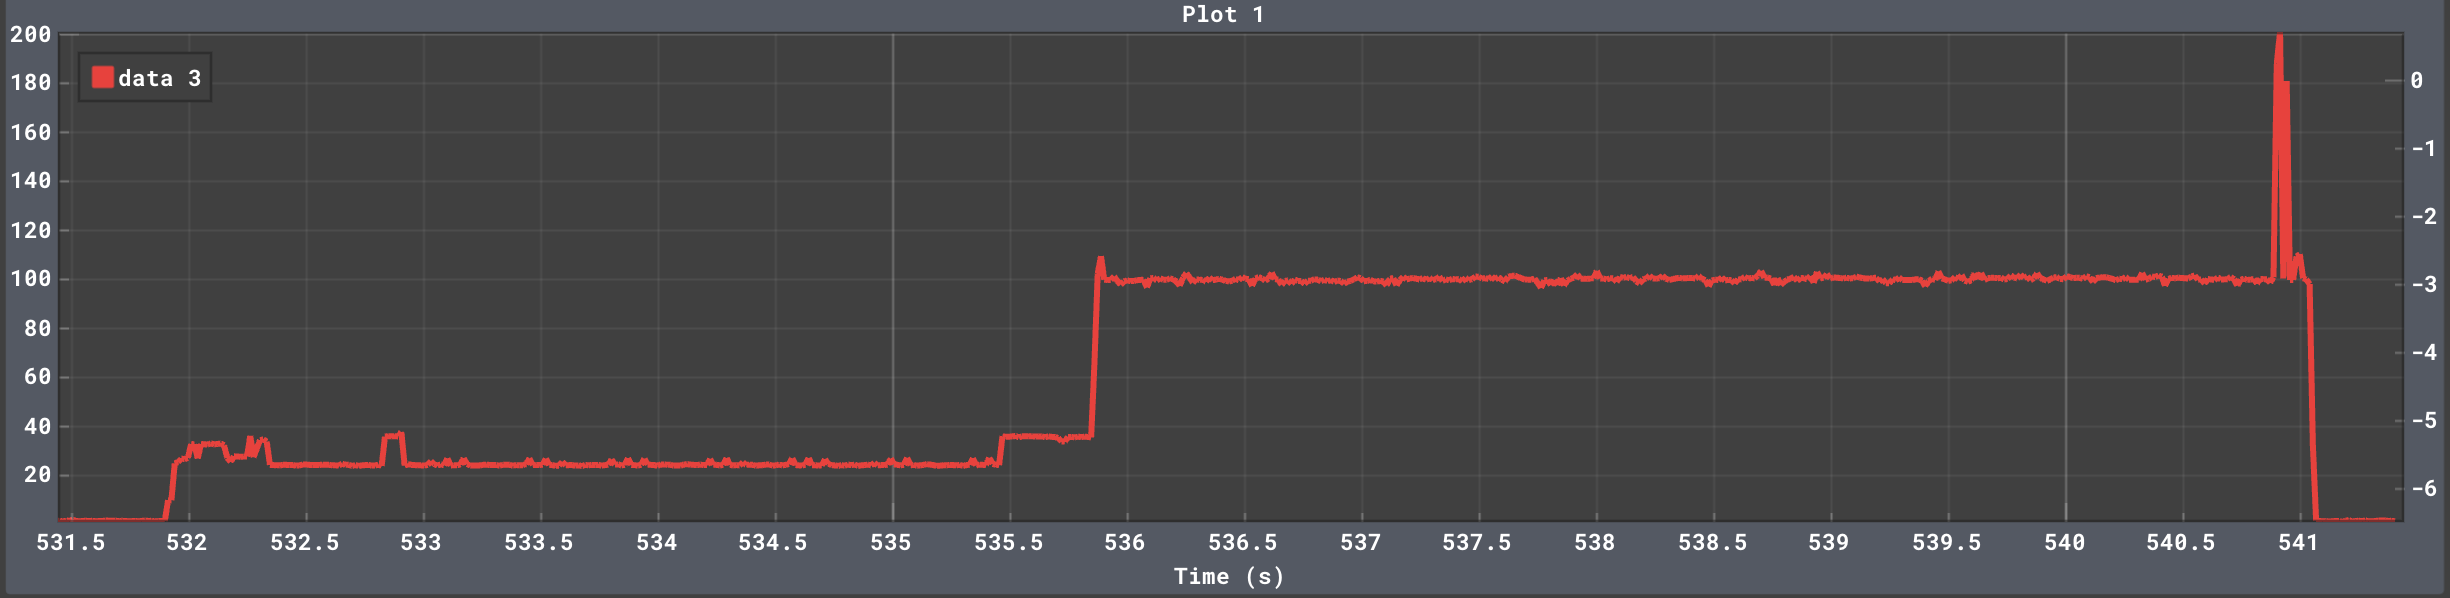
\includegraphics[width=\linewidth,keepaspectratio]{images/window energy with alarm detected.png}
  
  \vspace{0.2cm}
  {\scriptsize Signal energy over time during an active intrusion attempt. A rapid escalation in vibration intensity creates a major peak (reaching 200) that triggers the alarm classification.}
\end{column}
\hfill
\begin{column}{0.48\textwidth}
  \centering
  \textbf{\textcolor{sintefgreen}{No Alarm Detected}}
  
  \vspace{0.2cm}
  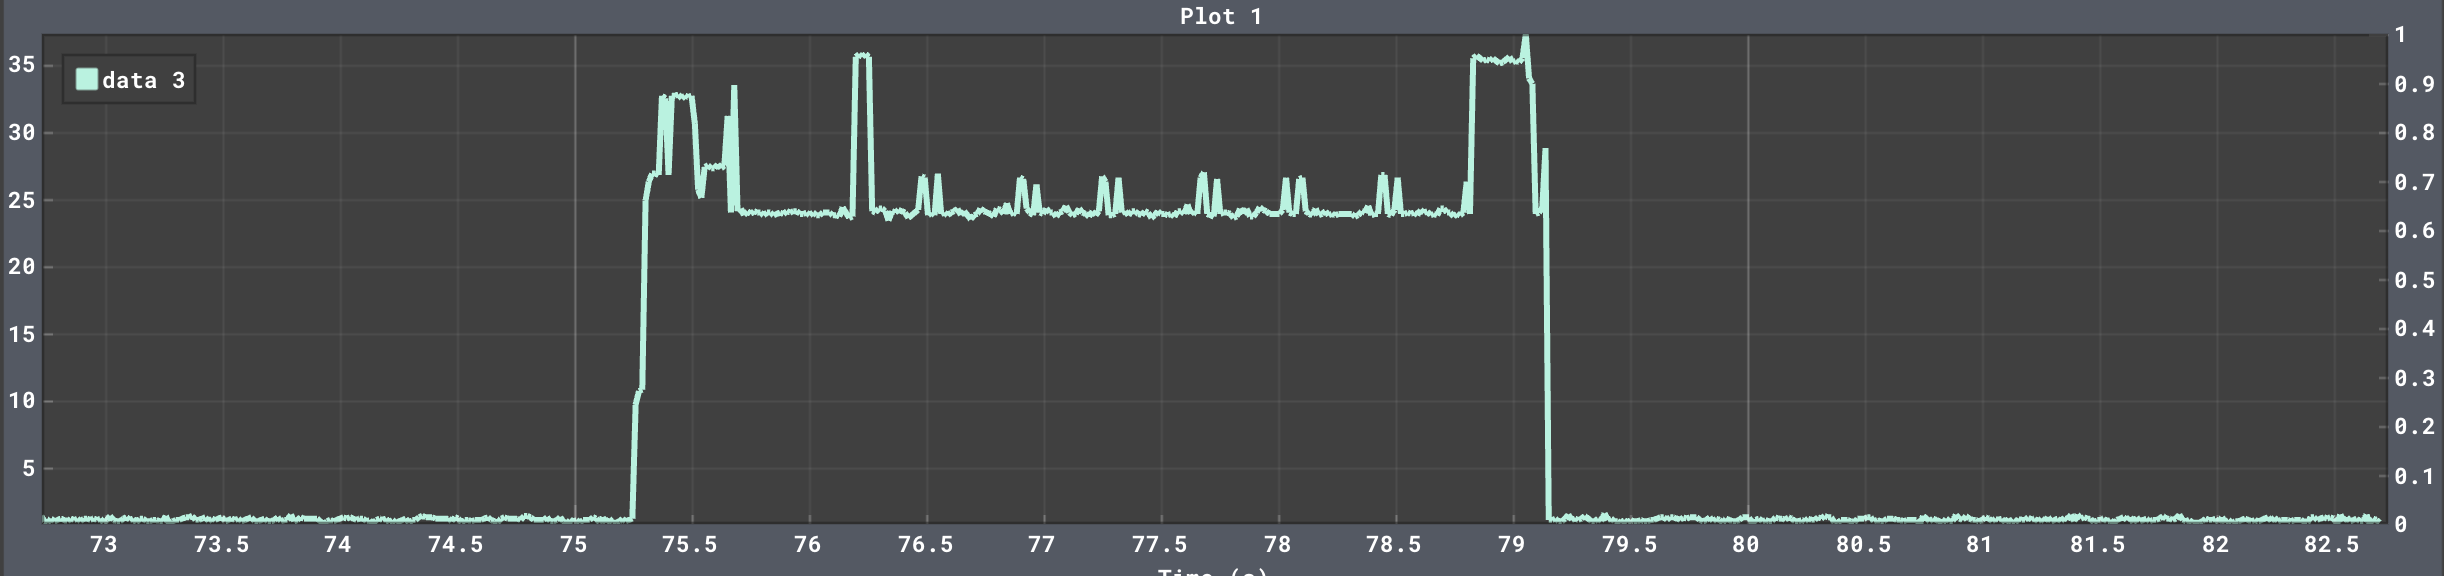
\includegraphics[width=\linewidth,keepaspectratio]{images/window energy with no alarm detected.png.png}
  
  \vspace{0.2cm}
  {\scriptsize Signal energy over time during ambient disturbances. The vibration remains within baseline limits (peaking around 35), which safely falls below the alarm threshold to prevent a false positive.}
\end{column}
\end{columns}
\end{frame}
